\raggedbottom
\chapter{Literature Review}

\section{Introduction}
There are many processes in science, management and technology that involves the rate of change of one variable in relation to another modeled as differential equations."Most differential equations in science and technology are solved by numerical methods"\cite{ross} because analytic solution is not possible ot useful \cite{lambert1977}.They are many existing algorithm designed for ODE such as Runge-kutta and Euler's Methods, Taylor series method \cite{lambert1977}, Hybrid methods by Ademiluyi(1987), Collocation method by Awoyemi(1996,1999 and 2000).However this paper addresses the use of linear multistep method to provide solutions to this differential problems.


One of the more challenging classes of problems in numerical computation is the solution of stiff equations and stiff systems. These problems arise from various physical situations but were likely first identified in chemical kinetics. Finding numerical solutions to stiff systems has been a significant challenge for numerical analysts. A potentially good numerical method for solutions of stiff systems must possess certain qualities in terms of its region of absolute stability and accuracy \cite{QURESH2024}.




\section{Exploring Stiff Systems of Ordinary Differential Equations: Characteristics, Solutions, and Numerical Methods}

Stiff ordinary differential equations (ODEs) pose significant challenges in scientific and engineering applications due to their unique properties, which can lead to numerical instability and inaccuracy in traditional numerical methods.Stiff ODEs are characterized by a rapid change in the solution over a short period, followed by a period of slow change. This characteristic can lead to numerical instability in traditional numerical methods, making it difficult to accurately solve these equations over long time scales.

The earliest detection of stiffness in differential equations in the digital computer era, by the two chemists, Curtiss and Hirschfelder \cite{curtisAndHirscfelder}, was apparently far in advance of its time. They named the phenomenon and spotted the nature of stiffness (stability requirement dictates the choice of the step size to be very small).To resolve the problem they recommended possible methods such as the Backward Differentiation Formula \cite{EMayers}




\subsection{Characteristics}
Stiff systems, in the realm of differential equations, possess specific mathematical characteristics that differentiate them from non-stiff systems. These characteristics often arise due to the underlying dynamics and structure of the system, particularly in the context of solving differential equations numerically. some of the main characteristics of stiff systems:

\begin{itemize}
  \item Multiple Time Scales: Stiff systems typically involve processes evolving at vastly different rates. Some components of the system change rapidly, while others evolve slowly. This time scale separation can lead to numerical stiffness, where traditional integration methods become inefficient or unstable.
  
  \item Eigenvalue Spectrum: Stiff systems exhibit eigenvalues with a wide range of magnitudes. This spectrum includes both large and small eigenvalues, with some eigenvalues dominating the behavior of the system. The presence of large eigenvalues relative to the integration step size contributes to stiffness.
  
  \item High Condition Number: Stiff systems often have matrices with high condition numbers. A high condition number indicates that the matrix is ill-conditioned, meaning small changes in the input can lead to large changes in the output. Ill-conditioning exacerbates numerical instability and error propagation.
  
  \item Exponential Dynamics: Stiff systems may contain components that exhibit rapid exponential growth or decay. These exponential dynamics can lead to numerical challenges, especially when using explicit integration methods that struggle to capture such behavior accurately.
  
  \item Implicitness Requirement: Stiff systems often necessitate the use of implicit numerical methods for stability. Implicit methods involve solving equations that relate the future state of the system to its current state. By incorporating future information, implicit methods can better handle stiff dynamics compared to their explicit counterparts.
  
  \item Small Stability Region: Stiff systems typically have a small stability region for explicit numerical methods. The stability region represents the range of integration parameters (e.g., step size) for which the numerical solution remains bounded. In stiff systems, the stability region can be severely limited, constraining the choice of integration parameters.
  
  \item Slow Transient Behavior: Despite the presence of fast processes, stiff systems may also exhibit slow transient behavior that requires accurate numerical representation. Balancing the resolution of fast and slow dynamics poses a challenge in numerical integration, particularly for stiff systems with widely varying time scales \cite{enwiki:1182900519}.
\end{itemize}

In this paper, we will be focusing on linear multistep methods to tackle this stiff property,  They are particularly well-suited for stiff systems due to their inherent stability properties and efficiency in handling multiple time scales.





Consider the initial value problem

\[
y'(x) = -15y(x), \quad x \geq 0, \quad y(0) = 1. \tag{1}
\]

The exact solution (shown in cyan) is

\[
y(x) = e^{-15x}, \quad y(x) \rightarrow 0 \text{ as } x \rightarrow \infty. \tag{2}
\]

We seek a numerical solution that exhibits the same behavior.

The figure (right) illustrates the numerical issues for various numerical integrators applied on the equation:
\begin{itemize}
    \item Euler's method with a step size of $h = \frac{1}{4}$ oscillates wildly and quickly exits the range of the graph (shown in red).
    \item Euler's method with half the step size, $h = \frac{1}{8}$, produces a solution within the graph boundaries but oscillates about zero (shown in green).
    \item The trapezoidal method (that is, the two-stage Adams–Moulton method) is given by
    \begin{equation}
      y_{n+1} = y_{n} + \frac{1}{2}h \left( f_{n} + f_{n+1} \right),
    \end{equation}

    where $y' = f(x,y)$. Applying this method instead of Euler's method gives a much better result (blue). The numerical results decrease monotonically to zero, just as the exact solution does.
\end{itemize}

Here is the image of stiff equation numerical solvers:

\begin{figure}[htbp]
  \centering
  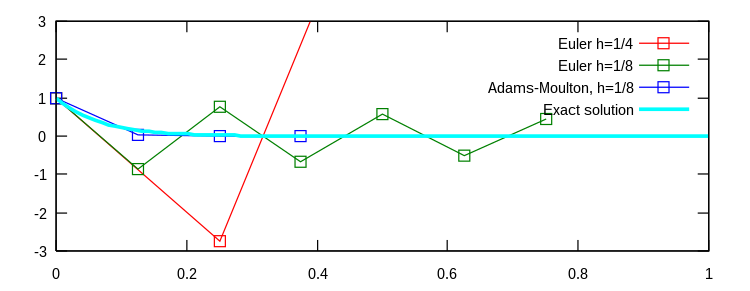
\includegraphics[width=0.8\textwidth]{chapters/2/StiffEquationNumericalSolvers.svg.png}
  \caption{Explicit numerical methods exhibiting instability when integrating a stiff ordinary differential equation}
  \label{fig:stiff_equation}
\end{figure}




\section{Multistep Methods}
Multistep methods are a category of numerical methods used to solve ordinary differential equations (ODEs), including stiff systems. They are called "multistep" because they use information from multiple previous steps to compute the next step. This makes them particularly effective for problems with stiff behavior, where the slope of the solution changes rapidly \cite{math7121158}.
One of the main strengths of multistep methods is their ability to handle temporal evolution. Because they use information from previous steps, they can adapt to changes in the behavior of the solution over time. This makes them particularly effective for problems where the solution evolves in a complex way, such as stiff systems \cite{math7121158}.

In terms of applications, multistep methods are widely used in various fields, including physics, engineering, and economics. They are used to solve a wide range of problems, from simulating the motion of celestial bodies to modeling economic growth. In the context of boundary value problems (BVPs), multistep methods can be used to solve problems where the solution varies over time and space \cite{math7121158}.

A general linear multistep method can be expressed as:

\begin{equation}
\sum_{j=0}^{k} \alpha_j y_{n+j} = h \sum_{j=0}^{k} \beta_j f(x_{n+j}, y_{n+j})
\end{equation}

where:


\begin{itemize}
  \item \(k\) is the number of previous steps to use
  \item \(h\) is the step length
  \item \(\alpha_j\) and \(\beta_j\) are the coefficients of the method
  \item \(y_{n+j}\) is the solution at the previous time steps
\end{itemize}


and also \[\alpha_k = 1, |\alpha_0| +| \beta_0 | \neq 0 \]

Linear multistep methods are generally defined by their coefficients \(\alpha_j\) and \(\beta_j\), and the choice of these coefficients determines the order and stability properties of the method. Common examples of linear multistep methods include the backward Euler method, the Adams-Bashforth methods, and the Adams-Moulton methods \cite{lambert1977}.


The solution at the next time step, \(y_{n+1}\), can be obtained by rearranging the terms in the above formula:


\begin{equation}
  y_{n+1} = \frac{1}{\alpha_0} \left(h \sum_{j=0}^{k} \beta_j f_{n+j} - \sum_{j=1}^{k} \alpha_j y_{n+j}\right)
\end{equation}


Linear multistep method can be classified into \textbf{Implicit} and \textbf{Explicit} LMM.


\subsection{Explicit Multistep Method}
Explicit linear multistep methods are a class of numerical methods used for solving ordinary differential equations (ODEs). These methods are designed to improve computational efficiency by utilizing information from previous steps in the solution process, rather than discarding it as in single-step methods like Euler's method \cite{enwiki:1182900519}.

The general form of an ELMM is give as:

\begin{equation}
  y_{n+1} = \sum_{j=0}^{k} \alpha_j y_{n+j} + h \sum_{j=0}^{k-1} \beta_j f_{n+j}
\end{equation}

Notice the $\beta_k = 0$, Hence a LMM in which $\beta_k = 0$ is called an Explicit LMM.

The key characteristic of explicit linear multistep methods is that they can directly compute the next value in the sequence without needing to solve for it, making them particularly useful for problems where computational resources are limited or where the solution needs to be obtained quickly.ELMM are also derived by  interpolating previously computed points and using this interpolation to compute future solution points \cite{Alexanderian2022}.

The Adams-Bashforth methods are a popular example of explicit linear multistep methods. They are used to solve ordinary differential equations (ODEs) and are particularly effective for non-stiff problems. The Adams-Bashforth methods are derived from the Lagrange interpolating polynomial and are used to approximate the solution at the next time step based on the solution at previous time steps.The Adams–Bashforth methods were designed by John Couch Adams to solve a differential equation modeling capillary action, and the theory was published by Francis Bashforth in 1883. These methods are widely used due to their efficiency and accuracy, especially for problems where the solution exhibits a strong dependency on the initial conditions \cite{enwiki:1166346639}. The Adams-Bashforth methods are widely used in scientific and engineering applications, including fluid dynamics, chemical kinetics, and climate modeling \cite{wong2020lecture}.

The general form of the Adams-Bashforth method of order $s$ is:

\begin{equation}
  y_{n+1} = y_n + h \sum_{j=0}^{s-1} b_j f_{n-j}
\end{equation}


where:

- $y_n$ is the known solution value at time step $t_n$,
- $h$ is the step size,
- $f_{n-j} = f(x_{n-j}, y_{n-j})$ are the derivative values at previous time steps, and
- $b_j$ are the method-specific coefficients.

The coefficients $b_j$ for the Adams-Bashforth methods are chosen such that the methods have order $s$. This means that the methods are accurate up to and including terms of order $h^s$ in the local truncation error.

The coefficients $b_j$ for the Adams-Bashforth methods are determined by the requirement that the method be consistent with the underlying differential equation and that it has the desired order of accuracy. Specifically, the coefficients are chosen such that the method reproduces the Taylor series expansion of the exact solution up to order $s$.

The Adams-Bashforth methods with $k=1,2,3,4,5$ respectively are given by \cite{butcher2003numerical} and \cite{hairer1993solving}:
\begin{align}
  y_{n+1} & = y_n + h \cdot f_n \\
  y_{n+2} & = y_{n+1} + h \left(\frac{3}{2}f_{n+1} - \frac{1}{2}f_{n}\right) \\
  y_{n+3} & = y_{n+2} + h \left(\frac{23}{12}f_{n+2} - \frac{4}{3}f_{n+1} + \frac{5}{12}f_{n}\right) \\
  y_{n+4} & = y_{n+3} + h \left(\frac{55}{24}f_{n+3} - \frac{59}{24}f_{n+2} + \frac{37}{24}f_{n+1} - \frac{9}{24}f_{n}\right) \\
  y_{n+5} & = y_{n+4} + h \left(\frac{1901}{720}f_{n+4} - \frac{2774}{720}f_{n+3} + \frac{2616}{720}f_{n+2} - \frac{1274}{720}f_{n+1} + \frac{251}{720}f_{n}\right)
\end{align}


\subsection{Implicit Multistep Method}
Implicit Linear Multistep Methods (ILMMs) are a class of numerical methods used for solving ordinary differential equations (ODEs) that are particularly advantageous in situations where the step size in an explicit method has to be chosen based on stability rather than accuracy \cite{alexander}.ILMMs are a subset of linear multistep methods (LMMs) that are used to solve ODEs by interpolating previously computed points and using this interpolation to compute future solution points. The key characteristic of ILMMs is that they require solving a nonlinear system of equations at each step, which makes them more stable than explicit methods, which can directly compute the next value in the sequence without needing to solve for it \cite{keller2020discovery}. In $(2.1)$, a LMM in which $\beta_k \neq 0$ is called an Implicit LMM.

In explicit methods, the step size is typically limited by the stability requirements imposed by the governing equations. For stiff ODEs, where there are rapid changes in the solution, explicit methods often necessitate very small step sizes to maintain stability. This can result in computationally expensive simulations, as a large number of steps are required to cover the solution domain adequately.

On the other hand, ILMMs allow for larger step sizes while maintaining stability, making them particularly advantageous for stiff ODEs. By implicitly incorporating information from future time steps, ILMMs can handle stiff problems more efficiently, reducing the computational cost associated with solving such equations.However, they can be more computationally expensive due to the need to solve a system of equations at each step \cite{thohura2013numerical}.

% Adams-Moulton method
One of the mostly widely used ILMMs is the Adams-Moulton method. The Adams-Moulton methods are a family of implicit linear multistep methods (ILMMs) commonly used for solving ordinary differential equations (ODEs). These methods are derived by considering the interpolation of the derivative function $f(x,y)$ over a given time interval.It is particularly advantageous for stiff systems, where explicit methods like the Adams-Bashforth method may require very small step sizes to maintain stability, leading to computationally expensive simulations. The Adams-Moulton method allows for larger step sizes while maintaining stability, making it more efficient for solving stiff ODEs.
The Adams-Moulton method is widely used in various scientific and engineering applications where accurate and stable numerical solutions of ODEs are required. It provides a balance between accuracy and computational efficiency, making it a valuable tool for simulating dynamic systems governed by differential equations.

The three-step Adams-Moulton method is given by:


\begin{equation}
  y_{n+3} = y_{n+2} + \frac{h}{24} \left( 9 f_{n+3} + 19 f_{n+2} - 5 f_{n+1} + f_{n} \right)
\end{equation}


This is the Adams-Moulton method of order 3, commonly denoted as AM(3). It is an implicit method because it requires solving for \( y_{n+1} \) implicitly in the equation. The method involves using the function values \( f_{n+3} \), \( f_{n+} \), and \( f_n \) to compute the value of \( y_{n+1} \), making it suitable for stiff ODEs where explicit methods may be unstable.


% Backward Differentiation Formula
Another implicit methods for stiff ODEs is the Backward Differentiation Formula (BDF).Backward Differentiation Formulas (BDFs) are a family of implicit numerical methods commonly used to solve stiff systems of ordinary differential equations (ODEs).BDFs use information from the future (at the next time level) to update the solution at the current time level. The backward nature of the method enables stability for stiff problems \cite{numericalrecipes}.

The general form of a BDF of order \(k\) is given by:

\begin{equation}
  \alpha_0 y_n + \alpha_1 y_{n-1} + \alpha_2 y_{n-2} + \ldots + \alpha_k y_{n-k} = h \cdot f_n
\end{equation}


It works by approximating the solution at the next step using a polynomial of degree less than or equal to the method order. This makes BDF suitable for stiff ODEs, as it avoids the loss of accuracy associated with steep slopes in the solution.BDFs are widely implemented in numerical software packages for solving stiff ODEs. Popular implementations include ode23s and ode45s \cite{shampine1997matlab},the Livermore Solver for Ordinary Differential Equations (LSODA),the Differential Algebraic System Solver (DASSL),GEAR, DIFSUB, and EPISODE \cite{Yatim2013} which is a collection of FORTRAN subroutines designed to facilitate the automated resolution of problems, minimizing the level of effort needed when encountering potential challenges in the problem-solving process \cite{thohura2013numerical}.


\subsection{Analysis of Multistep Method}

For a comprehensive analysis of linear multistep methods (LMMs), the paper titled "Linear Multistep Numerical Methods for Ordinary Differential Equations" by Nikesh S. Dattani is a valuable resource. This paper provides a review of the most popular LMMs, including the Adams-Bashforth Methods, Adams-Moulton Methods, and Backwards Differentiation Formulas. It discusses these methods in terms of their order, consistency, and various types of stability, offering a general overview that does not require much prior knowledge in numerical ODEs\cite{dattani2008linear}.

The general $k-step$ linear multistep method is given as 
\begin{equation}
  \alpha_k y_{n+k} + \alpha_{k-1} y_{n+k-1} + \ldots + \alpha_1 y_{n+1} + \alpha_0 y_n = h \left( \beta_k f_{n+k} + \beta_{k-1} f_{n+k-1} + \ldots + \beta_1 f_{n+1} + \beta_0 f_n \right)
\end{equation}

 which is equivalent to $(2.1)$, where $h$ is the parameter known as the \textbf{Step-size}, and $f_0, f_1, f_2 ... f_n$ are the values of the given function $f(x,y)$ at an equidistance of  $x_n = x_0 + nh$.

 The central concepts in the analysis of linear multistep methods, and indeed any numerical method for differential equations, are convergence, order, and stability. These concepts are crucial for understanding the behavior and performance of numerical methods in solving differential equations.

 \subsubsection*{Zero-Stability}
 Stability is a property that ensures the numerical solution does not explode or oscillate as the step size is reduced. A method is considered stable if it satisfies certain conditions related to the roots of the characteristic polynomial of the method. Specifically, all roots of the characteristic polynomial must lie inside the unit circle in the complex plane. This condition ensures that the method does not amplify errors and remains accurate as the step size is reduced \cite{wiki:analysis} \cite{Alexanderian2022}. A scheme that is zero-stable will not produce approximations which grow unrealistically with time.The stability of a numerical method is not as tangable as consistency and convergence but when you see an unstable solution it is obvious.

 The stability of multistep methods is determined by analyzing the roots of their characteristic polynomials. Methods that satisfy the root condition and have only one root with magnitude one are classified as strongly stable, while those with multiple distinct roots of magnitude one are termed weakly stable. Multistep methods that fail to meet the root condition are considered unstable \cite{butler_numerical_2022}.With this said it is safe to say that All one step methods, Adams-Bashforth and Adams-Moulton methods are all stongly stable.

 Given the \textbf{First characteristic polynomial} 
 \begin{equation}
  \rho(z) = \alpha_0 + \alpha_1 z + \alpha_2 z^2 + \dots + \alpha_k z^k
 \end{equation}

 where the $a_i$ are the coefficients of the LMM.
 LMM method are said to be \textbf{zero stable} if the zeros of the first characteristic polynomial such that

 \begin{enumerate}
  \item None of the zeros of the first characteristic polynomial are larger than 1 in magnitude.
  \item Any zero equal to 1 in magnitude is simple (i.e., not repeated).
\end{enumerate}

\subsubsection*{Convergence} 
Convergence refers to the property of a numerical method to produce a solution that approaches the exact solution as the step size approaches zero. A method is said to be convergent if the error between the numerical solution and the exact solution decreases as the step size is reduced. The rate of convergence is often expressed in terms of the order of the method, which indicates how quickly the error decreases with each step \cite{2022JFatokunEtAl}.


If the Linear multistep method satisfies the zero stable scheme and consistency scheme then it is said to be \textbf{convergent} \cite{2022JFatokunEtAl}.

\subsubsection*{Consistency and Order}
A scheme that is zero-stable will produce approximations that do not grow in size in a way that is not present in the exact, analytic solution. Zero stability is a required property, but it is not enough on its own. There remains the issue of whether the approximations are close to the exact values. The truncation error of the general linear multistep method is a measure of how well the differential equation and the numerical method agree with each other. It is defined by


\begin{equation}
  \tau_j = \frac{1}{\beta} \left( c_0 h y(jh) + c_1 y'(jh) + c_2 h y''(jh) + c_3 h^2 y'''(jh) + \ldots \right) = \beta h \sum_{p=0}^{\infty} c_p h^p y^{(p)}(jh)
\end{equation}
where $\beta = \sum \beta_j$ is a normalizing factor \cite{2022JFatokunEtAl}.
It is the first few terms in this expression that will matter most in what follows, and it helps us that there are formulae for the coefficients which appear:


\begin{equation}
  c_0 = \sum \alpha_j, \quad c_1 = \sum (j\alpha_j - \beta_j), \quad c_2 = \sum \left( j^2 \alpha_j - j \beta_j \right), \quad c_3 = \sum \left( \frac{j^3}{3!} \alpha_j - \frac{j^2}{2!} \beta_j \right)
\end{equation}
and so on. The general formula for $p \geq 2$ is

\begin{equation}
  c_p = \sum_{j=0}^{k} \left( \frac{(j^p)!}{p!} \alpha_j - \frac{(j^{p-1})}{(p-1)!} \beta_j \right),
\end{equation}

Recall that the truncation error is intended to be a measure of how well the differential equation and its approximation agree with each other\cite{HELM2008NumericalIVP}. In summary we can deduct that a linear multistep scheme is \textbf{consistent} if $c_0 = 0$ and $c_1 = 0$.


Assuming that the method is consistent, the order of the scheme tells us how quickly the truncation error tends to zero as $h \rightarrow 0$. For example, if $c_0 = 0$, $c_1 = 0$, $c_2 = 0$, and $c_3 \neq 0$, then the first nonzero term in $\tau_j$ will be the one involving $h^2$, and the linear multistep method is called second-order. This means that if $h$ is small, then $\tau_j$ is dominated by the $h^2$ term (because the $h^3$ and subsequent terms will be tiny in comparison), and halving $h$ will cause $\tau_j$ to decrease by a factor of approximately $\frac{1}{4}$. The decrease is only approximately known because the $h^3$ and other terms will have a small effect.In conclusion a linear multistep method is said to be of \textbf{order} $p$ if $c_0 = c_1 = c_2 = \ldots = c_p = 0$ and $c_{p+1} \neq 0$ \cite{HELM2008NumericalIVP}.




\subsection*{Numerical Solvers for Solving Stiff Systems}

However, like all numerical methods, multistep methods have their limitations. For example, they can suffer from numerical diffusion, where the solution becomes smoother than expected due to roundoff errors. This can lead to inaccuracies in the solution, especially for problems with stiff behavior. Furthermore, the choice of the number of previous steps to use can significantly affect the performance of the method. More steps can lead to more accurate solutions, but they also increase the computational cost \cite{math7121158}.

The \texttt{ode15s} and \texttt{ode23} solvers in MATLAB are examples of multistep methods used for solving stiff systems of BVPs or IVPs. The \texttt{ode15s} solver uses an implicit Runge-Kutta method of order 15, with the embedded 6th order BDF method as a predictor. It is able to handle stiff and nonstiff problems and can be used with either the Jacobian of the system or a numerical approximation. On the other hand, the \texttt{ode23} solver uses an implicit Runge-Kutta method of order 2, with the embedded 3rd order BDF method as a predictor. It is also able to handle stiff and nonstiff problems \cite{wong2020lecture}.

The \texttt{bvp4c} and \texttt{bvp5c} solvers in MATLAB are examples of multistep methods used for solving BVPs. They use a collocation method with a finite difference code that implements the Lobatto IIIa formula. This is a collocation formula, and the collocation polynomial provides a $C^1$-continuous solution that is fourth-order or fifth-order accurate uniformly in the interval of integration.

Each of these tools has its strengths and weaknesses; \texttt{DIFSUB} has no graphical user interface, which makes it harder for users who are not comfortable working from the command-line or with text-based interfaces, and it is a very old package, therefore finding support becomes challenging; \texttt{GEAR} uses a FORTRAN package, users need to have some knowledge of FORTRAN to use it effectively; \texttt{EPISODE} is a deprecated package which performs faster than \texttt{GEAR} in solving waves or active solutions, but the reverse for linear or decaying problems \cite{BYRNE1977125}. With these limitations comes the aim of this project.

The Runge-Kutta-Fehlberg (RKF45) method is another widely used implicit method for solving ordinary differential equations, including stiff ODEs. It combines both explicit and implicit methods to achieve high accuracy and stability \cite{stone2017accelerating}.

\[
\begin{aligned}
  k_1 & = h \cdot f(x_n, y_n), \\
  k_2 & = h \cdot f\left(x_n + \frac{1}{4}h, y_n + \frac{1}{4}k_1\right), \\
  k_3 & = h \cdot f\left(x_n + \frac{3}{8}h, y_n + \frac{3}{32}k_1 + \frac{9}{32}k_2\right), \\
  k_4 & = h \cdot f\left(x_n + \frac{12}{13}h, y_n + \frac{1932}{2197}k_1 - \frac{7200}{2197}k_2 + \frac{7296}{2197}k_3\right), \\
  k_5 & = h \cdot f\left(x_n + h, y_n + \frac{439}{216}k_1 - 8k_2 + \frac{3680}{513}k_3 - \frac{845}{4104}k_4\right), \\
  k_6 & = h \cdot f\left(x_n + \frac{1}{2}h, y_n - \frac{8}{27}k_1 + 2k_2 - \frac{3544}{2565}k_3 + \frac{1859}{4104}k_4 - \frac{11}{40}k_5\right).
\end{aligned}
\]

\[
y_{n+1} = y_n + \frac{16}{135}k_1 + \frac{6656}{12825}k_3 + \frac{28561}{56430}k_4 - \frac{9}{50}k_5 + \frac{2}{55}k_6.
\]

\[
\text{Error} = \frac{1}{360}h(-127k_1 + 845k_3 - 28561k_4 + 9k_5 - 2k_6).
\]

Although there exist no specific stiff system solver that utilizes the RKF45 method exclusively, the RKF45 method is a variant of the Dormand-Prince method, which is a popular implicit Runge-Kutta method used in MATLAB's \texttt{ode15s} solver \cite{BurkardtRKF45}. It's worth noting that while the RKF45 method is not used by a specific stiff system solver, it is a powerful tool for solving stiff systems of ODEs. Its ability to accurately estimate the local truncation error and adapt the step size accordingly allows it to handle stiff problems effectively \cite{BurkardtRKF45}.

  

\section{Collocation Methods}
Collocation methods are a class of numerical methods used to solve ordinary differential equations (ODEs), including stiff systems. They work by choosing specific points (collocation points) within the domain where the solution is sought. The solution is then approximated as a polynomial at these points, and the differential equation is converted into a set of algebraic equations by enforcing the equations at these points.
Numerous studies have demonstrated the efficacy of collocation methods in various scientific and engineering applications. Examples include the modeling of chemical reactions, structural dynamics, and climate phenomena. The ability of collocation methods to efficiently capture rapid changes in the system dynamics makes them well-suited for problems characterized by stiff components.
In the realm of stiff systems, collocation methods exhibit notable advantages, offering enhanced efficiency by directly manipulating the coefficients of the differential equation, ensuring heightened accuracy in capturing stiff behavior, and providing increased stability; however, their implementation complexity and sensitivity to the choice of collocation points present challenges\cite{Faleichik2009ExplicitIO}.

Let's consider a simple second-order ordinary differential equation (ODE) as an example:

\[
y''(x) = f(x, y, y')
\]

with boundary conditions \(y(a) = \alpha\) and \(y(b) = \beta\). The objective is to find the function \(y(x)\) that satisfies the differential equation and boundary conditions.

The collocation method involves selecting a set of collocation points \(\{x_1, x_2, \ldots, x_n\}\) within the domain \([a, b]\). At these collocation points, the differential equation is enforced. This results in a system of algebraic equations that can be solved to obtain the values of \(y(x_i)\) at the collocation points.

Let \(y_i = y(x_i)\) and \(y_i' = y'(x_i)\). Applying the collocation method to the differential equation, we have:

\[
y_i'' = f(x_i, y_i, y_i')
\]

This equation is enforced at each collocation point \(x_i\), resulting in a set of algebraic equations:

\[
y_1'' = f(x_1, y_1, y_1')
\]
\[
y_2'' = f(x_2, y_2, y_2')
\]
\[
\vdots
\]
\[
y_n'' = f(x_n, y_n, y_n')
\]

 The accuracy and stability of the collocation method depend on the choice of collocation points and the method used to solve the resulting system of equations.



